%!TEX root = ../sbc-template.tex

\emph{Smart} TV é tida como um aparelho de televisão com capacidades interativas ligadas à internet, como aplicativos disponíveis em lojas; acesso a conteúdo online como notícias, previsão do tempo, informações de mercados de ações, mapas e jogos; \emph{e-commerce}; navegação web e acesso a redes sociais\cite{shin2013smart}. Estes aparelhos podem ser equipadas com câmeras e microfones embutidos\cite{michele2014watch}, além de óculos 3D \cite{perakakis2015proposed}, como mostra a Figura \ref{fig:smart_samsung}. Estas televisões utilizam os mesmos sistemas operacionais e conjuntos de aplicativos que computadores comuns, o que as torna sucetíveis às mesmas falhas e ataques de segurança que outros dispositivos semelhates \cite{michele2014watch}.
\begin{figure}
	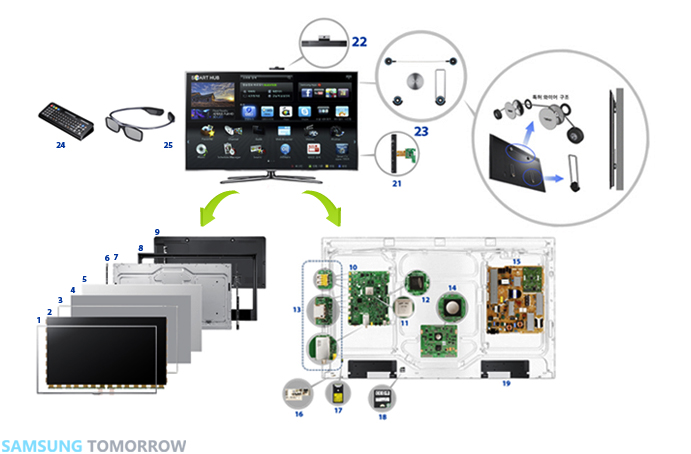
\includegraphics[width=\textwidth]{img/smart_samsung.jpg}
	\caption{\emph{Smart} TV Samsung}
	\label{fig:smart_samsung}
\end{figure}
